% For LaTeX-Box: root = stat105_F15_exam1B.tex 
%%%%%%%%%%%%%%%%%%%%%%%%%%%%%%%%%%%%%%%%%%%%%%%%%%%%%%%%%%%%%%%%%%%%%%%%%%%%%%%%
%  File Name: stat105_F15_exam1B.tex
%  Purpose:
%
%  Creation Date: 24-09-2015
%  Last Modified: Thu Feb 18 05:20:37 2016
%  Created By:
%%%%%%%%%%%%%%%%%%%%%%%%%%%%%%%%%%%%%%%%%%%%%%%%%%%%%%%%%%%%%%%%%%%%%%%%%%%%%%%%
\documentclass[addpoints]{examsetup}\usepackage[]{graphicx}\usepackage[]{color}
%% maxwidth is the original width if it is less than linewidth
%% otherwise use linewidth (to make sure the graphics do not exceed the margin)
\makeatletter
\def\maxwidth{ %
  \ifdim\Gin@nat@width>\linewidth
    \linewidth
  \else
    \Gin@nat@width
  \fi
}
\makeatother

\definecolor{fgcolor}{rgb}{0.345, 0.345, 0.345}
\newcommand{\hlnum}[1]{\textcolor[rgb]{0.686,0.059,0.569}{#1}}%
\newcommand{\hlstr}[1]{\textcolor[rgb]{0.192,0.494,0.8}{#1}}%
\newcommand{\hlcom}[1]{\textcolor[rgb]{0.678,0.584,0.686}{\textit{#1}}}%
\newcommand{\hlopt}[1]{\textcolor[rgb]{0,0,0}{#1}}%
\newcommand{\hlstd}[1]{\textcolor[rgb]{0.345,0.345,0.345}{#1}}%
\newcommand{\hlkwa}[1]{\textcolor[rgb]{0.161,0.373,0.58}{\textbf{#1}}}%
\newcommand{\hlkwb}[1]{\textcolor[rgb]{0.69,0.353,0.396}{#1}}%
\newcommand{\hlkwc}[1]{\textcolor[rgb]{0.333,0.667,0.333}{#1}}%
\newcommand{\hlkwd}[1]{\textcolor[rgb]{0.737,0.353,0.396}{\textbf{#1}}}%

\usepackage{framed}
\makeatletter
\newenvironment{kframe}{%
 \def\at@end@of@kframe{}%
 \ifinner\ifhmode%
  \def\at@end@of@kframe{\end{minipage}}%
  \begin{minipage}{\columnwidth}%
 \fi\fi%
 \def\FrameCommand##1{\hskip\@totalleftmargin \hskip-\fboxsep
 \colorbox{shadecolor}{##1}\hskip-\fboxsep
     % There is no \\@totalrightmargin, so:
     \hskip-\linewidth \hskip-\@totalleftmargin \hskip\columnwidth}%
 \MakeFramed {\advance\hsize-\width
   \@totalleftmargin\z@ \linewidth\hsize
   \@setminipage}}%
 {\par\unskip\endMakeFramed%
 \at@end@of@kframe}
\makeatother

\definecolor{shadecolor}{rgb}{.97, .97, .97}
\definecolor{messagecolor}{rgb}{0, 0, 0}
\definecolor{warningcolor}{rgb}{1, 0, 1}
\definecolor{errorcolor}{rgb}{1, 0, 0}
\newenvironment{knitrout}{}{} % an empty environment to be redefined in TeX

\usepackage{alltt}

\usepackage{etoolbox}
\usepackage{tikz,pgfplots}

%% For LaTeX-Box: root = stat105_exam1_info.tex 
%%%%%%%%%%%%%%%%%%%%%%%%%%%%%%%%%%%%%%%%%%%%%%%%%%%%%%%%%%%%%%%%%%%%%%%%%%%%%%%%
%  File Name: stat105_exam1_info.tex
%  Purpose:
%
%  Creation Date: 24-09-2015
%  Last Modified: Thu Sep 24 13:51:36 2015
%  Created By:
%%%%%%%%%%%%%%%%%%%%%%%%%%%%%%%%%%%%%%%%%%%%%%%%%%%%%%%%%%%%%%%%%%%%%%%%%%%%%%%%
\newcommand{\course}[1]{\ifstrempty{#1}{STAT 105}{STAT 105, Section #1}}
\newcommand{\sectionNumber}{B}
\newcommand{\examDate}{October 1, 2015}
\newcommand{\semester}{FALL 2015}
\newcommand{\examNumber}{II}

\newcommand{\examTitle}{Exam \examNumber}

\runningheader{\course{\sectionNumber}}{Exam \examNumber}{\examDate}
\runningfooter{}{}{Page \thepage of \numpages}

\newcommand{\examCoverPage}{
   \begin{coverpages}
   \centering
   {\bfseries\scshape\Huge Exam I \par}
   \vspace{1cm}
   {\bfseries\scshape\LARGE \course{\sectionNumber} \par}
   {\bfseries\scshape\LARGE \semester \par}

   \vspace{2cm}

   \fbox{\fbox{\parbox{5.5in}{\centering 

      \vspace{.25cm} 
      
      {\bfseries\Large Instructions} \\

      \vspace{.5cm} 

      \begin{itemize}
         \item  The exam is scheduled for 80 minutes, from 8:00 to 9:20 AM. At 9:20 AM the exam will end.\\
         \item  A forumula sheet is attached to the end of the exam. Feel free to tear it off.\\
         \item  You may use a calculator during this exam.\\
         \item  Answer the questions in the space provided. If you run out of room, continue on the back of the page. \\
         \item  If you have any questions about, or need clarification on the meaning of an item on this exam, please ask your instructor. No other form of external help is permitted attempting to receive help or provide help to others will be considered cheating.\\
         \item  {\bfseries Do not cheat on this exam.} Academic integrity demands an honest and fair testing environment. Cheating will not be tolerated and will result in an immediate score of 0 on the exam and an incident report will be submitted to the dean's office.\\
      \end{itemize}

   }}}

   \vspace{2cm}

   \makebox[0.6\textwidth]{Name:\enspace\hrulefill}

   \vspace{1cm}

   \makebox[0.6\textwidth]{Student ID:\enspace\hrulefill}
   \end{coverpages}

}


\newcommand{\course}[1]{\ifstrempty{#1}{STAT 105}{STAT 105, Section #1}}
\newcommand{\sectionNumber}{A}
\newcommand{\examDate}{February 18, 2016}
\newcommand{\semester}{SPRING 2016}
\newcommand{\examNumber}{I}

%%%%%%%%%%%%%%%%%%%%%%%%%%%%%%%%%%%%%%%%%%%%%%%%%%%%%%%%%%%%%%%%%%%%%%%%%%%%%%%%
\IfFileExists{upquote.sty}{\usepackage{upquote}}{}
\begin{document}

%-- : R code (Code in Document)



\examCoverPage

\begin{questions}

\question

%-- question1: R code (Code in Document)


\textbf{Netflix recommendations}

A Recommender System is a statistical tool many websites use to recommend new items, products, or services to a user based on the user's history.
For example, the popular movie streaming service Netflix recommends movies a user might like by assigning a predicting a rating between 0 and 5 to movies the user has not previously rated on the site and recommending the movies with the highest predicted rating.
Netflix is testing a few changes in their recommendation system in an attempt to increase its accuracy.
A specific user's true ratings are recorded below as well as the predicted ratings from the current recommender system and the predicted ratings from the new recommender system:


% latex table generated in R 3.1.3 by xtable 1.7-4 package
% Thu Feb 18 05:20:40 2016
\begin{table}[ht]
\centering
\begin{tabular}{rrrrrrrrrrr}
   & \multicolumn{10}{c}{Ratings} \\
User's True Ratings & 4.30 & 4.10 & 4.10 & 4.20 & 4.20 & 4.20 & 4.30 & 4.30 & 4.20 & 4.20 \\ 
  Current System Predictions & 4.50 & 4.20 & 3.70 & 4.80 & 4.30 & 4.00 & 4.40 & 3.80 & 4.40 & 3.70 \\ 
  New System Predictions & 0.40 & 0.20 & 0.20 & 0.30 & 0.30 & 0.30 & 0.40 & 0.40 & 0.30 & 0.30 \\ 
  \end{tabular}
\end{table}



\begin{parts}

   \part[2] Is the new recommender system more or less accurate than the current system?

   \vspace{1cm}

   \part[2] Is there a possible calibration-like adjustment that would improve the accuracy of either system? Expain.

   \vspace{1cm}

\end{parts}

\question 
\textbf{Chilling fluid}

The production of a certain type of metal beam involves rapidly cooling the beam to 10 degrees Celsius by submerging it in a bath of chilling fluid.
The time required to reduce the beams temperature should be short or the cooling process can cause problems on the production line.
During a single working week, six beams were randomly chosen and the time it took to cool them to 10 degrees Celsius is recorded below (in minutes):


$$
   12.1, 12.8, 13.3, 13.4, 14, 14.2
$$

Using these observed values, report the following:

\begin{parts}

   \part[2] the mean  
   \vspace{1cm}

   \part[2] the variance 
   \vspace{1cm}

   \part[2] the standard deviation 
   \vspace{1cm}

   \part[2] the value of $Q(.30)$
   \vspace{1cm}

   \part[2] the interquartile range
   \vspace{1cm}

\end{parts}

\newpage

\question

\textbf{Coloring books}

Power4People (P4P), an electical utility company, has consulted with workplace psychologists to find ways to reduce the stress levels of their engineering employees.
The psychologists recommended two techniques: (1) practicing transcendental meditation and (2) spending time on simple arts and crafts projects.
P4P has asked one of their engineers, KW, to determine which (if either) of two techniques is most effective.
P4P's engineers belong to one of three departments: computing (22 engineers); electical (26 engineers); and construction (30 engineers).
It is believed that stress levels will be different for each department (for instance, the computer engineers travel less frequently).
The psychologists have created an exam that measures stress levels from 0 (lowest) to 100 (highest), with all scores between 0 and 100 possible.

After a little thought, KW comes up with the following plan:
18 engineers are randomly selected from each of the three departments. 
All the selected engineers take the exam to measure their stress level.
The 18 engineers selected from each department are then randomly split into three groups of six engineers each.
\begin{itemize}
   \item The first group will meet each morning from 10:00 to 10:30 to practice transcendental meditation,
   \item The second group will meet each morning from 10:00 to 10:30 to quietly color in the coloring books,
   \item The third group will have no adjustment to their work schedule.
\end{itemize}
After two weeks, the engineers are again given the exam to measure their stress level and the change in their stress level is recorded.

\begin{parts}

  \part[3] Is this an experiment or an observational study? Explain.

  \vspace{2cm}

  \part For each of the following variables types, identify whether it is numeric or qualitative. If it is numeric, state whether it is continuous or discrete. If it qualitative, provide the possible values. 

  \vspace{.5cm}

   \begin{subparts}

      \subpart[3] Response variable(s) (if there is no response variable, put ``Not Used"):

      \vspace{2cm}

      \subpart[3] Experimental variable(s) (if there is no experimental variable, put ``Not Used"):

      \vspace{2cm}

      \subpart[3] Controlled variable(s) (if there is no control variable, put ``Not Used"):

      \vspace{2cm}

      \subpart[3] Blocking variable(s) (if there is no blocking, put ``Not Used"):

      \vspace{2cm}

   \end{subparts}

\end{parts}

\pagebreak

\question

\textbf{Tidal torrents}

Within 24 hours of its release, The Life of Pablo, a new album by Kanye West, had been illegally downloaded over 500,000 times by people using BitTorrent,
a system in which users download a file to their own computers and upload the file to the computers of others.

For one hour, starting at 6:00 pm and continuing until 7:00 pm Eastern, 
a systems engineer working for the company that stands to lose money from the piracy used a combination of tools to gather the following information on every 
500th individual who began downloading a torrent of the album.

\begin{itemize}
   \item Whether the individual was in the United States or not,
   \item The individual's average upload speed,
   \item The individual's average download speed,
   \item The number of users the individual shared the album with,
\end{itemize}

Tidal plans to use the data gathered to illustrate the extent of their loss in future legal action.

\begin{parts}

   \part[2] Is this an experiment or an observational study?

   \vspace{2cm}

   \part[2] What is the population being considered?

   \vspace{2cm}

   \part It turns out that average upload speed and average download speed were very strongly, positively, correlated. Answer each of the following TRUE or FALSE.

   \vspace{0.5cm}

      \begin{subparts}

         \subpart[1]   We can conclude that higher values of average \textbf{download} speed \textit{cause} the value of average \textbf{upload} speed to be \textbf{higher}.

         \vspace{0.5cm}
         
         \subpart[1]   We can conclude that higher values of average \textbf{download} speed \textit{cause} the value of average \textbf{upload} speed to be \textbf{lower}.

         \vspace{0.5cm}
         
         \subpart[1]   We can conclude that higher values of average \textbf{upload} speed \textit{cause} the value of average \textbf{download} speed to be \textbf{higher}.

         \vspace{0.5cm}

         \subpart[1]   We can conclude that higher values of average \textbf{upload} speed \textit{cause} the value of average \textbf{download} speed to be \textbf{lower}.

      \end{subparts}

   \vspace{1cm}

   \part[2] After noticing that most of the users are from the United States, one executive comments that most Kanye West fans are Americans. 
            Another executive points out that most of Europe is asleep at 6:00 pm eastern and wouldn't be awake to download the album.
            In this case, whether or not a person is awake could be considered what kind of variable?

\end{parts}
\pagebreak

\question 

\textbf{Highlights}

%-- : R code (Code in Document)


The lifetime of a highlighter can be measured in the area of paper it can cover with highlighting fluid until either the marker falls apart or it runs out of highlighter fluid.
A sample of 26 highlighters were used until the end of their lifetime. The areas covered by the highlighters (in square meters) are recorded below:

%-- : R code (Code in Document)
\begin{knitrout}
\definecolor{shadecolor}{rgb}{0.969, 0.969, 0.969}\color{fgcolor}\begin{kframe}
\begin{verbatim}

  The decimal point is at the |

  0 | 1
  1 | 28
  2 | 7
  3 | 113588
  4 | 055688
  5 | 011789
  6 | 9
  7 | 0
  8 | 
  9 | 24
\end{verbatim}
\end{kframe}
\end{knitrout}

Note that \verb!1 | 9! represents 1.9. In this case, the first quartile is $Q(.25) = 3.3$, 
the median is 4.55, and the third quartile is $Q(.75) = 5.7$.

\begin{parts}
  \part[10] Complete the following frequency table: \\

  \begin{table}[h!]
     \centering
     \begin{tabular}{|l|p{3cm}|p{3cm}|p{4cm}|}
        \hline
                             & \textbf{Frequency} & \textbf{Relative} & \textbf{Cumulative}  \\
        \textbf{Value Range} &                    & \textbf{Frequency} & \textbf{Relative Frequency} \\\hline \hline
                    &  &  &  \\
      0.00 - 2.00   &  &  &  \\
                    &  &  &  \\ \hline
                    &  &  &  \\
      2.01 - 4.00   &  &  &  \\
                    &  &  &  \\ \hline
                    &  &  &  \\
      4.01 - 6.00   &  &  &  \\
                    &  &  &  \\ \hline
                    &  &  &  \\
      6.01 - 8.00   &  &  &  \\
                    &  &  &  \\ \hline
                    &  &  &  \\
      8.01 - 10.00  &  &  &  \\
                    &  &  &  \\ \hline
     \end{tabular}
  \end{table}
  \newpage

  \part[5] Using the area below, create a \textbf{dot plot} to summarize the data. 


%-- : R plot (results in document)
\begin{knitrout}
\definecolor{shadecolor}{rgb}{0.969, 0.969, 0.969}\color{fgcolor}
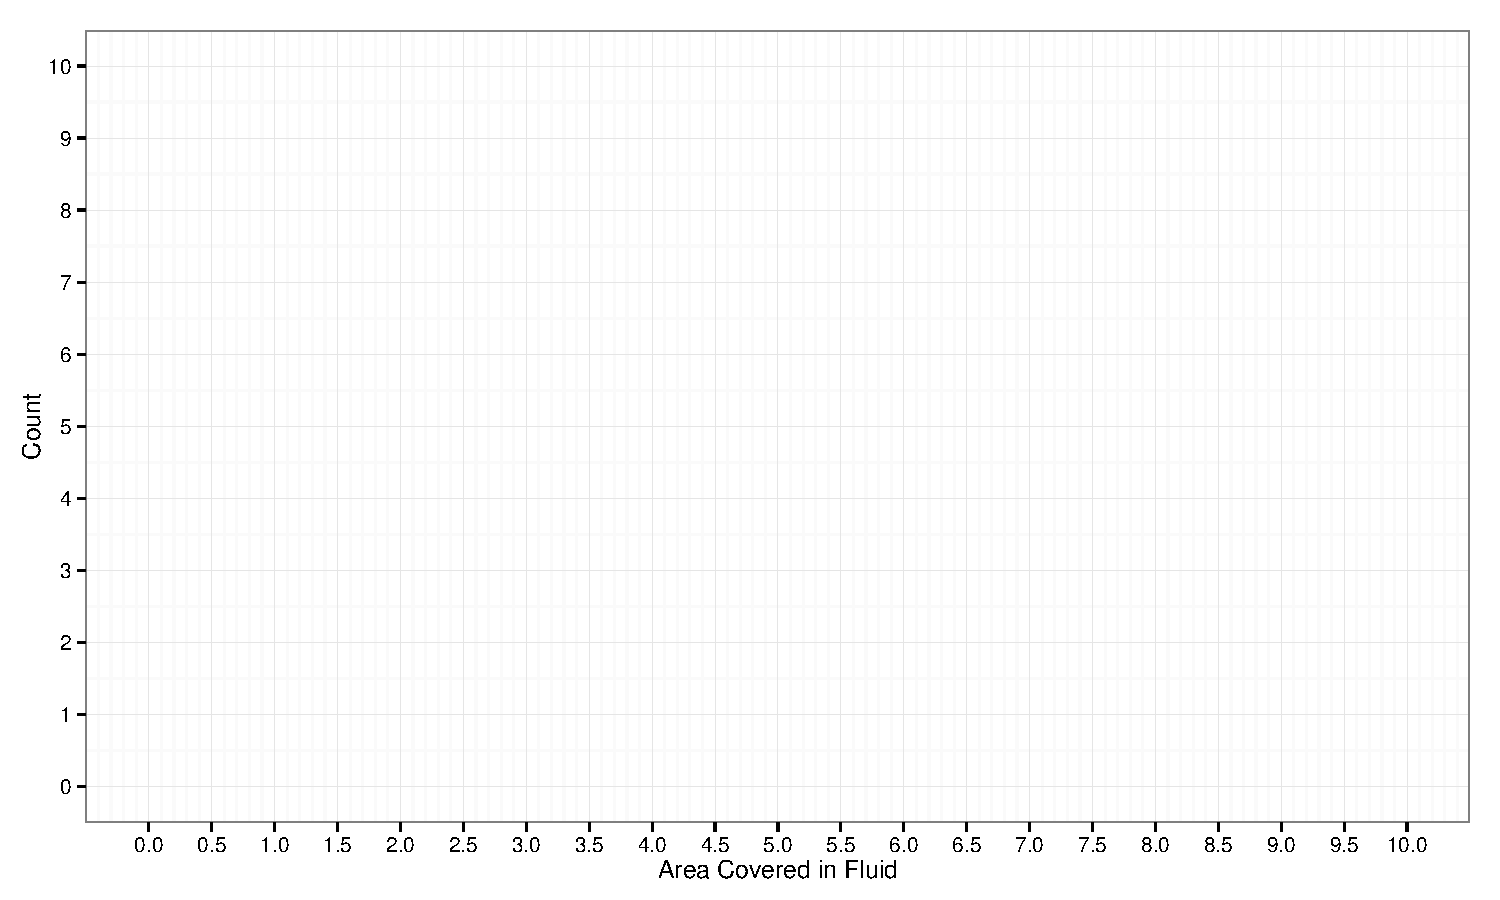
\includegraphics[width=1.1\linewidth]{figure/unnamed-chunk-6-1} 

\end{knitrout}

  \part[10] Using the area below, create a \textbf{box plot} to summarize the data.  Carefully label the important parts. 

%-- : R plot (results in document)
\begin{knitrout}
\definecolor{shadecolor}{rgb}{0.969, 0.969, 0.969}\color{fgcolor}
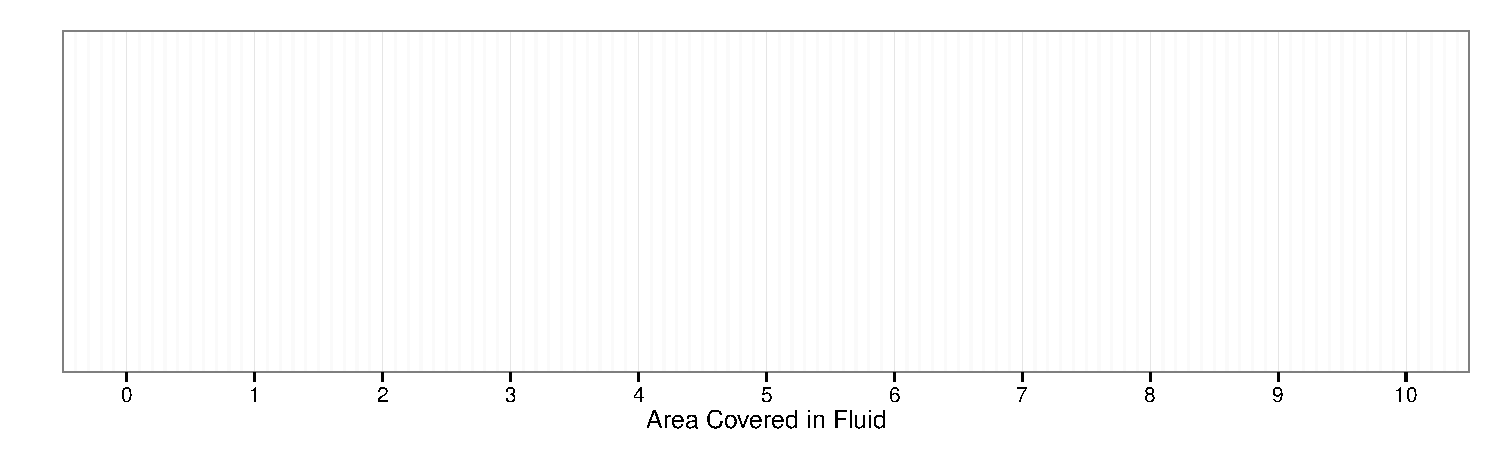
\includegraphics[width=\linewidth]{figure/unnamed-chunk-7-1} 

\end{knitrout}

  \part[4] Are there any unusually low or high observations? If so, what was the area covered by those highlighters?

\end{parts}
\pagebreak

\question

\textbf{Ultralight beams}

An ultralight beam is a type of metal beam used as secondary support in the facade of tall structures. 
Its low weight and high flexibility make it ideal for environments exposed to high amounts of pressure.

A manufacturer of ultralight beams performed the following analysis to illustrate the flexible nature of the beams.
26 ultralight beams were fixed in place vertically.
Each beam had a different amount of force applied to it, from 5 kN 55 kN, for 20 minutes in an attempt to bend the bar.
After the twenty minutes, the beam had a chance to ``bounce back" the final displacement from its original position was measured (in centi-radians).
The smaller the displacement, the better the bar did in returning to its original position.

The experiment was repeated, this time using the steel beams traditionally used as secondary support in the facade of tall buildings (referred to from here on as ``traditional beams").

%-- : R code (Code in Document)


The results are depicted below (with the force applied on the x-axis, and with ultralight beam observations represented with triangles and traditional beam results represented by dots):

\begin{center}
\begin{knitrout}
\definecolor{shadecolor}{rgb}{0.969, 0.969, 0.969}\color{fgcolor}
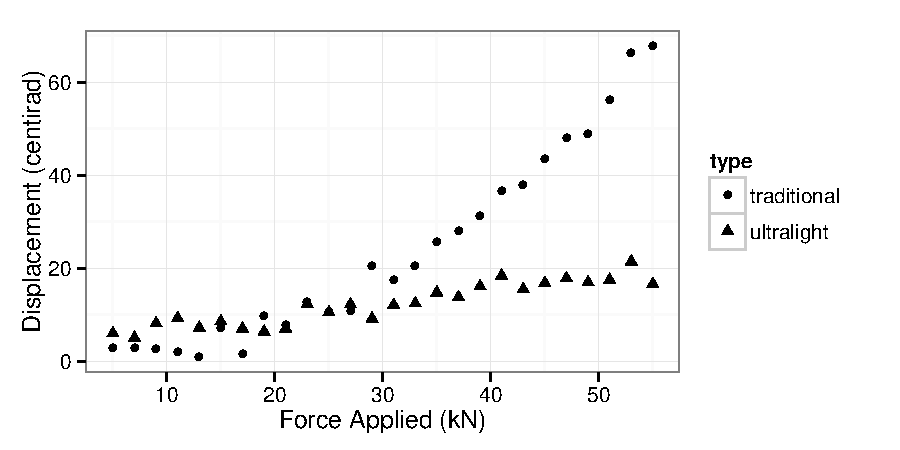
\includegraphics[width=.8\linewidth]{figure/unnamed-chunk-9-1} 

\end{knitrout}
\end{center}

Here are some summaries of the ultralight data (again using the force applied as the x-value and the displacement of the beam as the y-value):

$$
   \sum_{i=1}^{50} x_i = 780 \hspace{3cm} \sum_{i=1}^{50} x_i^2 = 29250 \\
$$

$$
   \sum_{i=1}^{50} y_i = 319 \hspace{3cm} \sum_{i=1}^{50} y_i^2 = 4455 \\
$$

$$
   \sum_{i=1}^{50} x_i y_i = 11227
$$

\newpage
\begin{parts}
   \part Using the summaries above, we plan to fit a linear relationship between \textbf{force applied} (x) and \textbf{displacement} (y) for the ultralight beam. 
   \begin{subparts}
      \subpart[5] Write the equation of the fitted linear relationship. 
      \vspace{2cm}
      \subpart[5] Find and interpret the value of $R^2$ for the fitted linear relationship.
      \vspace{2cm}
      \subpart[5] Using the fitted line, what do we suppose the displacement of an ultralight beam will be if the force applied is 41.
      \vspace{2cm}
      \subpart[5] The ultralight beam that actually underwent 41 kN had a displacement of 18.41 centiradians. What is the residual associated with this observation?
      \vspace{2cm}
   \end{subparts}

   \newpage 

   \part The JMP output below comes from fitting a quadratic model using the force applied (\verb!force_app!) and the square of the force applied (\verb!force_app^2!) for the displacement of the traditional beams.

   \centerline{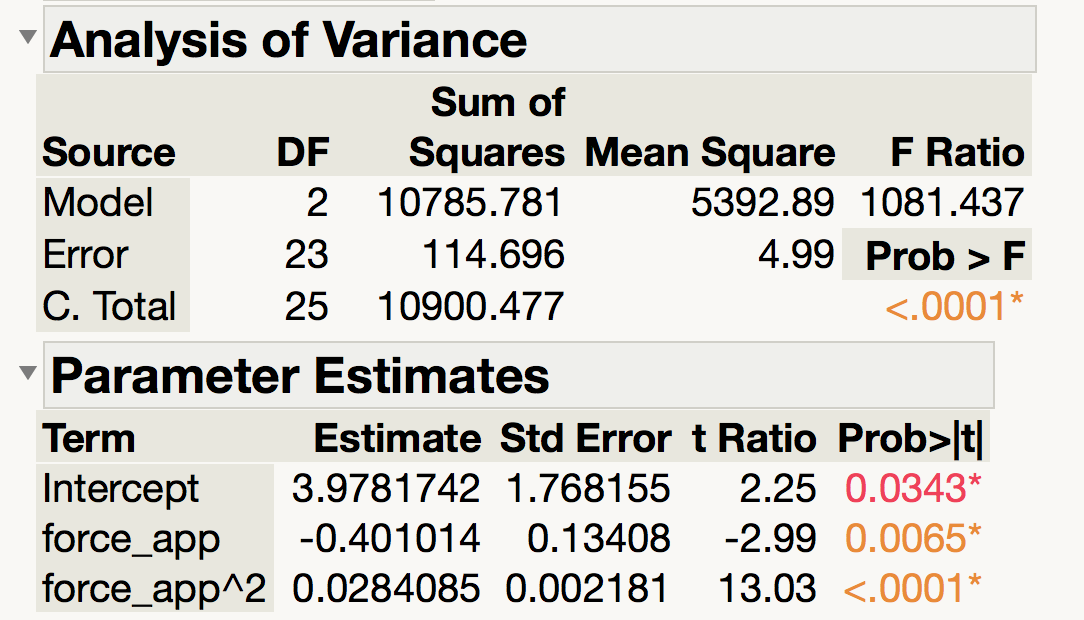
\includegraphics[scale=.5]{square_fit}}

   \begin{subparts}
      \subpart[5] Write the equation of the fitted quadratic relationship.
      \vspace{2cm}
      \subpart[5] Find and interpret the value of $R^2$ for the fitted quadratic relationship.
      \vspace{2cm}
      \subpart[5] Using the fitted line, what do we suppose the displacement of an traditional beam will be if the force applied is 41.
      \vspace{2cm}
      \subpart[5] The traditional beam that actually underwent 41 kN had a displacement of 36.68 centiradians. What is the residual associated with this observation?
      \vspace{2cm}
   \end{subparts}
\end{parts}

\end{questions}

\end{document}
